\subsubsection{The Forced Undamped Pendulum}
We add the external force to the expression for $\varphi^{\prime\prime}$.
We assume that this force is periodic in the time $t$, even that it has a simple cosine shape.
\begin{equation}
	\varphi^{\prime\prime}=-\omega^2\sin\varphi+A\cos\Omega t
\end{equation}
We show two motions in the diagrams of Figure (\ref{fig:tfcup}).
In both cases, $\Omega=1, A=0.01, \varphi(0)=0.017, \varphi^\prime(0)=0$, and the time interval is $[0,200]$.
The free pendulum oscillates with a well-defined frequency and also the forcing has a well-defined frequency.
In the motions depicted in Figure (\ref{fig:tfcup}) both frequencies remain visible. Like \emph{multi} or \emph{quasi}\emph{-periodic} motion (Section (\ref{sec:paqp})). 
\begin{figure}[h!]
	\centering
	\begin{subfigure}{0.45\linewidth}
		\centering
		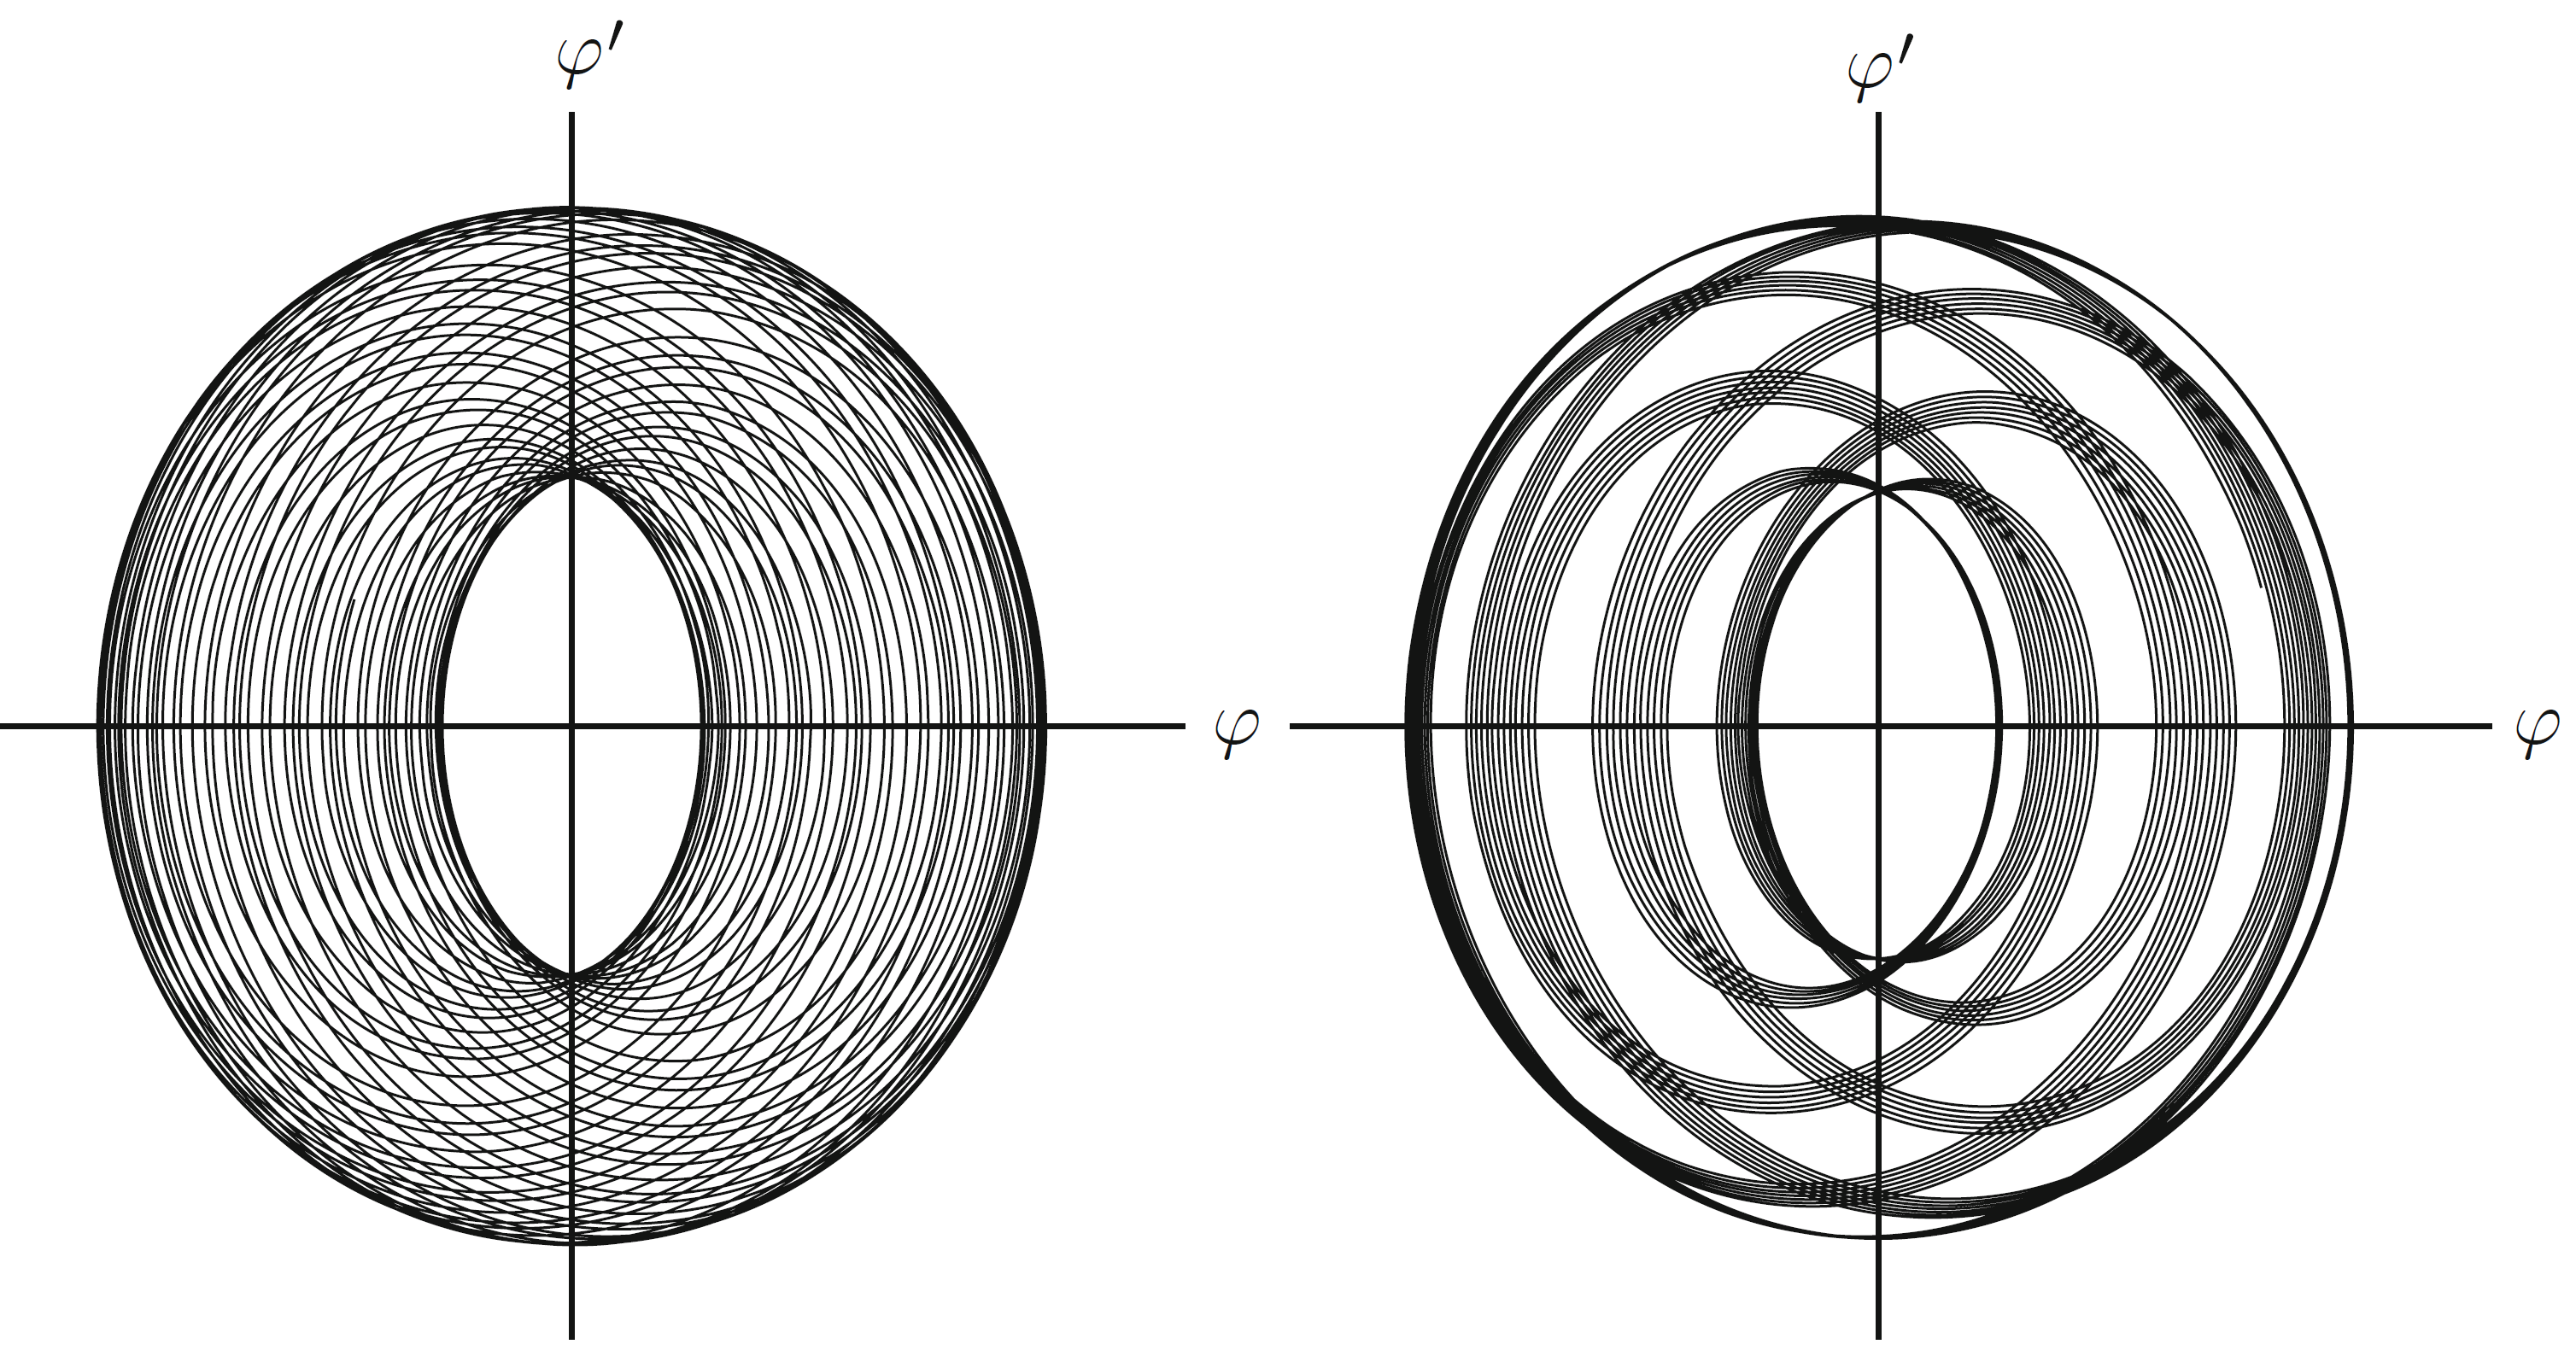
\includegraphics[width=\linewidth]{tfcup.png}
		\caption{Two multiperiodic evolutions of the periodically forced undamped pendulum.\\
		Left: $\omega=\frac{1}{2}(1+\sqrt{5})\approx1.61803$ (golden ratio).\\
		Right: $\omega=$1.602}
		\label{fig:tfcup}
	\end{subfigure}
	\vline
	\begin{subfigure}{0.52\linewidth}
		\centering
		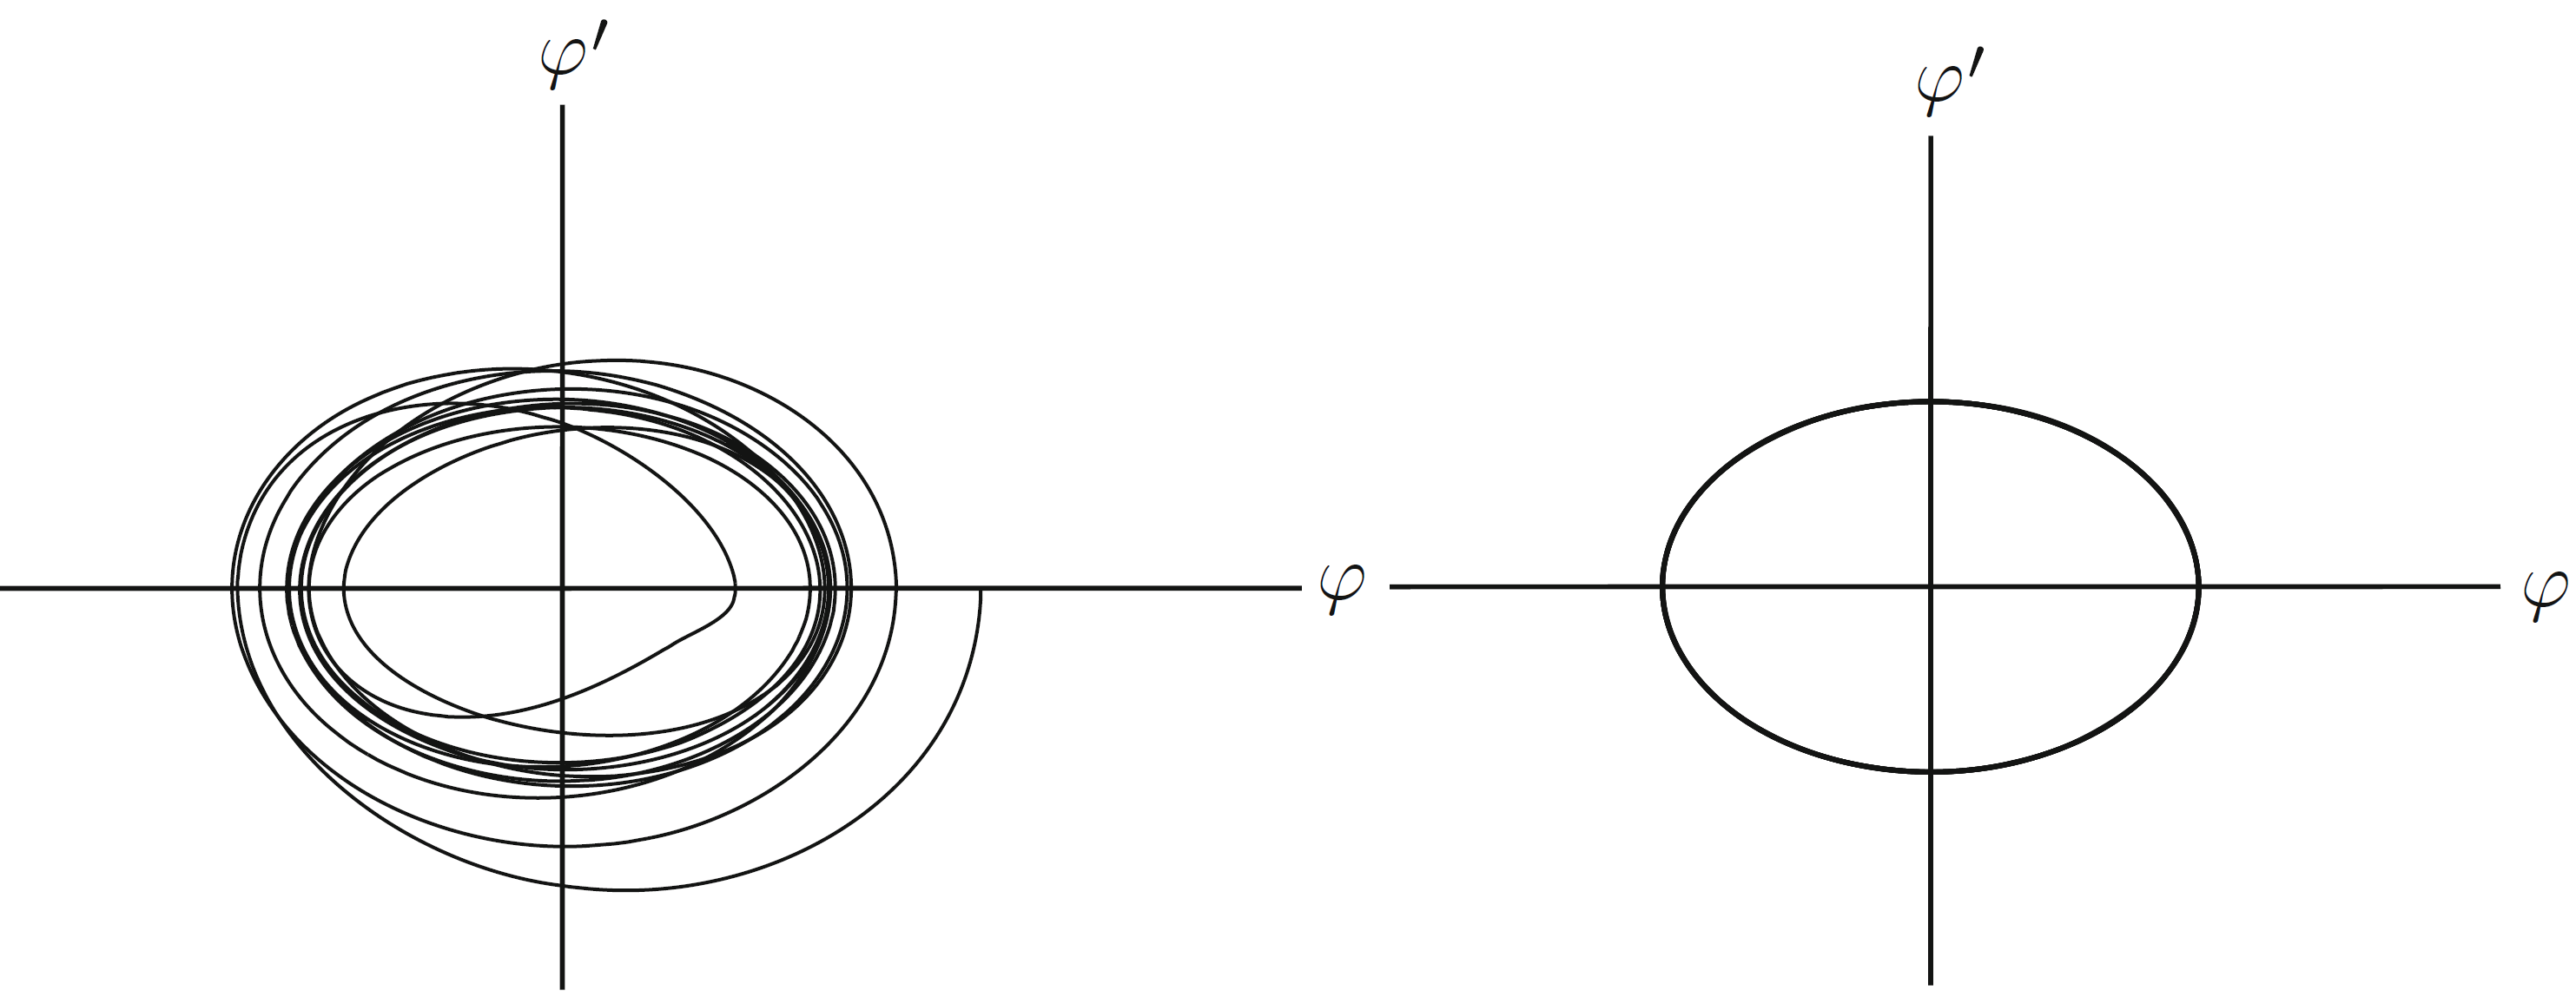
\includegraphics[width=\linewidth]{tfcdp.png}
		\caption{Evolution of the damped and forced pendulum as $t$-parametrised curve.\\
		Left: $t\in[0,100]$, the evolution tends to a periodic motion.\\
		Right: t>100, continuation of the segment in the left diagram.}
		\label{fig:tfcdp}
	\end{subfigure}
	\caption{}
\end{figure}
\subsubsection{The Forced Damped Pendulum}
Adding damping, we arrive at the following equation of motion
\begin{equation}{\label{eq:tfcdp}}
	\varphi^{\prime\prime}=-\omega^2\sin\varphi-c\ \varphi^\prime+A\cos\Omega t
\end{equation}
In Figure (\ref{fig:tfcdp}) we took $\omega=1.43, \Omega=1, A=0.2, c=0.1$ and $\varphi(0)=0.3, \varphi^\prime(0)=0$ we show an example of a motion of the damped forced pendulum (\ref{eq:tfcdp}), that only after a long time (say about 100 time units) tends to a periodic motion. 
It can be shown that the system, with equation of motion (\ref{eq:tfcdp}) with well-chosen values of the parameters $\omega$, $c$, $A$ and $\Omega$, has motions that never tend to a periodic motion, i.e. \emph{Chaos}.